\section{1174070 - Arrizal Furqona Gifary}
Chapter 8 - Perkenalan Generative Adversarial Network
\subsection{Teori}
\subsubsection{Jelaskan dengan ilustrasi gambar sendiri apa itu generator dengan perumpamaan anda sebagai mahasiswa sebagai generatornya.}
\hfill\\
\begin{figure}[H]
	\centering
	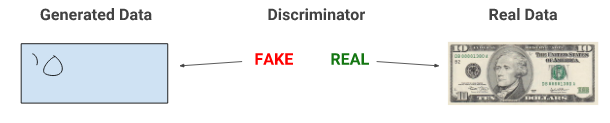
\includegraphics[width=8cm]{figures/1174070/8/gan_diagram.png}
	\caption{gambaran penjelasan no. 1}
\end{figure}
\begin{figure}[H]
	\centering
	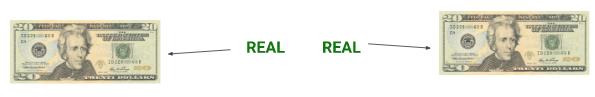
\includegraphics[width=8cm]{figures/1174070/8/gan_diagram2.png}
	\caption{gambaran penjelasan no. 1}
\end{figure}
Pertama, mahasiswa akan mencoba untuk meniru data asli seperti gambar diatas yaitu uang dengan cara menggambarnya, sekilas memang terlihat sangat jelas perbedaan antara keduanya dan disini pihak discriminator yaitu dosen akan mampu untuk membedakan gambar yang digambar oleh mahasiswa dengan data asli, setelah itu mahasiswa akan mencoba berulang kali hingga data yang ditirunya mirip seperti pada gambar kedua, bila dilihat pada gambar kedua sangat mirip sekali antara satu sama lain sehingga pihak discriminator kesulitan membedakannya dan melabelinya sebagai data real.

\subsubsection{Jelaskan dengan ilustrasi gambar sendiri apa itu diskriminator dengan perumpamaan dosen anda sebagai diskriminatornya.}
\begin{figure}[H]
	\centering
	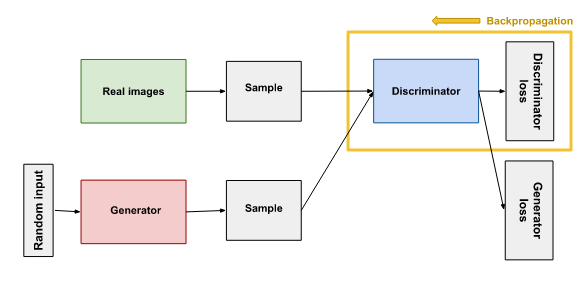
\includegraphics[width=8cm]{figures/1174070/8/discriminator.png}
	\caption{gambaran penjelasan no. 2}
\end{figure}
\hfill\\
Diskriminator sederhananya adalah suatu hal yang digunakan untuk melakukan klasifikasi yang membedakan data asli dengan data yang di hasilkan oleh generator, disini dosen bisa digambarkan sebagai seorang diskriminator yang mengevaluasi tiap mahasiswanya, misalkan mahasiswa menggambar suatu tiruan dari data A, nah dosen akan mampu membedakan gambar yang asli dengan gambar yang dibuat oleh mahasiswa karena dosen sudah memiliki klasifikasinya tersendiri


\subsubsection{Jelaskan dengan ilustrasi gambar sendiri bagaimana arsitektur generator dibuat}
\hfill\\
Arsitektur GAN, terdiri dari generator yang menghasilkan data sample dan juga ada data asli yang dijadikan sampel kemudian diinputkan ke discriminator yang kemudian akan melabeli data mana yang real dan tiruan
\begin{figure}[H]
	\centering
	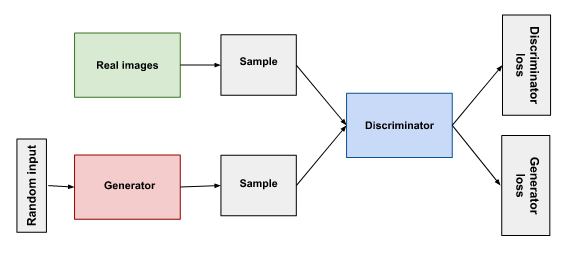
\includegraphics[width=8cm]{figures/1174070/8/arsitektur_GAN.png}
	\caption{gambar arsitektur generator pada GAN-Project}
\end{figure}


\subsubsection{Jelaskan dengan ilustrasi gambar sendiri bagaimana arsitektur generator dibuat}
\hfill\\
Arsitektur GAN, terdiri dari generator yang menghasilkan data sample dan juga ada data asli yang dijadikan sampel kemudian diinputkan ke discriminator yang kemudian akan melabeli data mana yang real dan tiruan
\begin{figure}[H]
	\centering
	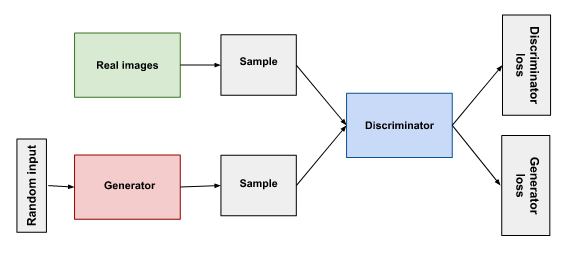
\includegraphics[width=8cm]{figures/1174070/8/arsitektur_GAN.png}
	\caption{gambar arsitektur generator pada GAN-Project}
\end{figure}

\subsubsection{Jelaskan dengan ilustrasi gambar apa itu latent space.}
\hfill\\
Latent space sederhananya adalah bentuk representasi dari data yang di compress, bisa dibilang di machine learning pun kita perlu melakukan optimisasi data dengan cara melakukan compress pada data yang akan kita gunakan agar sizenya tidak terlalu besar
\begin{figure}[H]
	\centering
	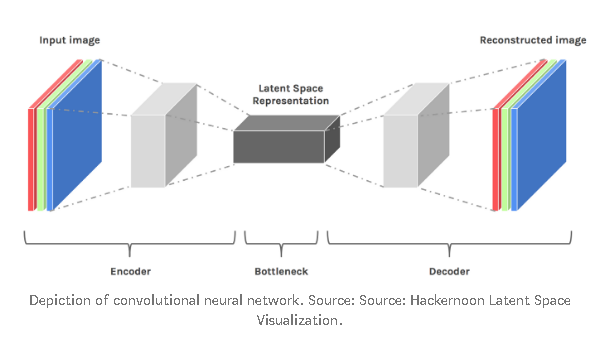
\includegraphics[width=8cm]{figures/1174070/8/latentspace.png}
	\caption{gambaran penjelasan no. 5}
\end{figure}

\subsubsection{Jelaskan dengan ilustrasi gambar apa itu adversarial play}
\hfill\\
Merupakan proses yang terjadi antara generator dengan diskriminator dalam gan untuk membuat diskriminator salah dalam melabeli suatu data.
\begin{figure}[H]
	\centering
	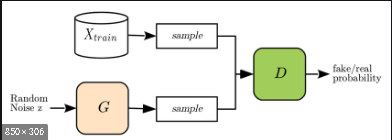
\includegraphics[width=10cm]{figures/1174070/8/adversarialplay.png}
	\caption{gambaran penjelasan no. 6}
\end{figure}

\subsubsection{Jelaskan dengan ilustrasi gambar apa itu Nash equilibrium}
\hfill\\
Suatu situasi stabil dari suatu sistem yang berkaitan dengan interaksi dari banyak partisipan, dimana tidak ada satupun orang yang bisa mengganti strateginya jika yang lain tidak menggantinya juga
\begin{figure}[H]
	\centering
	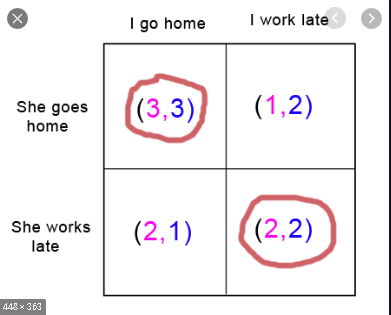
\includegraphics[width=10cm]{figures/1174070/8/nash.png}
	\caption{gambaran penjelasan no. 7}
\end{figure}

\subsubsection{Sebutkan dan jelaskan contoh-contoh implementasi dari GAN}
\hfill\\
Contonnya adalah sebagai berikut, mereka adalah orang orang yang dihasilkan oleh algoritma ini, alias tidak ada di dunia ini.

\begin{figure}[H]
	\centering
	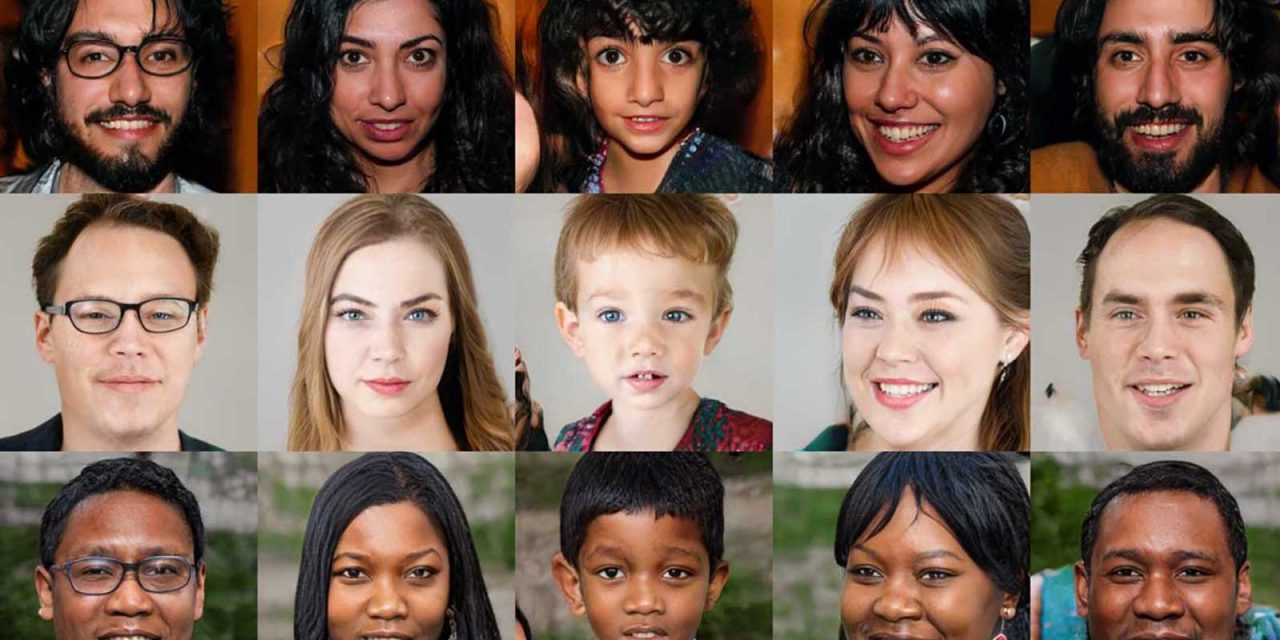
\includegraphics[width=10cm]{figures/1174070/8/implementasigan.jpg}
	\caption{gambaran penjelasan no. 8}
\end{figure}

\subsubsection{Berikan contoh dengan penjelasan kode program beserta gambar arsitektur untuk membuat generator(neural network) dengan sebuah input layer, tiga hidden layer(dense layer), dan satu output layer(reshape layer)}
\hfill\\
Berikut adalah kode programnya, untuk gambar sudah di sertakan di nomor sebelumnya
\lstinputlisting[firstline=8, lastline=20, caption={Kode program arsitektur generator},captionpos=b]{src/1174070/8/teori.py}

\subsubsection{Berikan contoh dengan ilustrasi dari arsitektur dikriminator dengan sebuath input layer, 3 buah hidden layer, dan satu output layer.}
\hfill\\
untuk gambar arsitektur nya ada pada gambar no. 4 sedangkan untuk kode programnya seperti berikut:
\lstinputlisting[firstline=23, lastline=35, caption={Kode program arsitektur diskriminator},captionpos=b]{src/1174070/8/teori.py}


\subsubsection{Jelaskan bagaimana kaitan output dan input antara generator dan diskriminator tersebut. Jelaskan kenapa inputan dan outputan seperti itu.}
\hfill\\
Kaitannya antara output dengan input adalah pelabelan data, generator akan terus berusaha menghasilkan data fake yang pada akhirnya karena sangat mirip maka discriminator akan melabelinya asli.

\subsubsection{Jelaskan apa perbedaan antara Kullback-Leibler divergence (KL divergence)/relative entropy, Jensen-Shannon(JS) divergence / information radius(iRaD) / total divergence to the average dalam mengukur kualitas dari model.}
\hfill\\
Kullback–Leibler divergence mengukur bagaimana suatu distribusi probabilitas berbeda dari yang kedua, dari kedua algoritma diatas, yang paling umum diketahui oleh banyak orang adalah KL divergence, kl divergence memiliki beberapa sisi bagus contohnya adalah KL[q; p] jenis daerah yang di mana q(x) memiliki massa non-null dan p(x) memiliki massa null. memang terlihat seperti bug ,tetapi dalam situasi tertentu ini adalah fitur. dan JS tidak memilikinya,

\subsubsection{Jelaskan apa itu fungsi objektif yang berfungsi untuk mengukur kesamaan antara gambar yang dibuat dengan yang asli.} 
\hfill\\
fungsi objektif adalah suatu fungsi yang akan mengambil beberapa parameter di suatu data dan juga model yang kemudian dijadikan argumen untuk dievaluasi, sehingga nantinya akan mengembalikan angka yang mampu membedakan antara gambar asli dan palsu.

\subsubsection{Jelaskan apa itu scoring algoritma selain mean square error atau cross entropy seperti The Inception Score dan The Frechet Inception distance.} 
\hfill\\
Inception score digunakan untuk mengukur kualitas dari gambar yang digenerated, khususnya yang tiruan,sintetik seperti yang dihasilkan algoritma GAN, sedangkan Frechet Inception distance digunakan untuk mengukur dua data set gambar, berkaitan sekali dengan kualitas visual manusia dalam menentukan gambar, dan algoritma ini sering digunakan di GAN
\subsubsection{Jelaskan kelebihan dan kekurangan GAN} 
\hfill\\
\begin{itemize}
 \item Kelebihan 
   \begin{enumerate}
      \item GAN  merupakan metode bagus untuk melakukan training classifier dalam metode semi supervised
      \item GAN melakukan proses generate yang cepat dibandingkan dengan metode lainnya.
      \item GAN tidak butuh pengukuran monte carlo
      \item GAN lebih mudah digunakan dibandingkan dengan VAE
   \end{enumerate}
 \item Kekurangan
   \begin{enumerate}  
      \item Melakukan training gan membutuhkan kita untuk mencari nash quilibrium
      \item Agak sulit untuk generate data text
      \item Dibandingkan dengan boltzmann machine, gan sulit untuk menebak value dari suatu pixel
      \item Sangat sensitif dengan data yang sudah diinisiasi sebelumnya
   \end{enumerate}
\end{itemize}

\subsection{Praktek}
\subsubsection{Jelaskan apa itu 3D convolutions}
\hfill\\
3D convolutions merupakan operasi konvolusi 3D yang menerapkan filter 3D ke data input dengan tiga arah, yaitu x,y, dan z. fitur ini menciptakan sebuah daftar peta yang ditumpuk. agar lebih mudah saya menggunakan sebuah ilustrasi seperti berikut:
\begin{figure}[H]
	\centering
	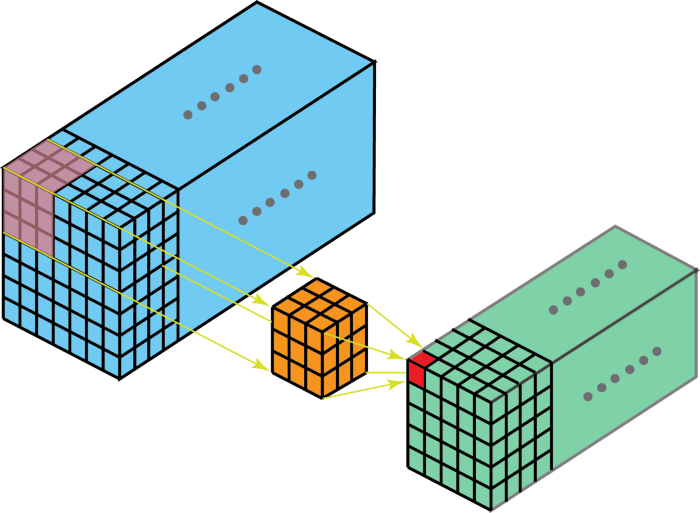
\includegraphics[scale=0.5]{figures/1174070/8/3dconvolutions.png}
	\caption{gambaran 3D Convolutions}
\end{figure}

\subsubsection{Jelaskan dengan kode program arsitektur dari generator networknya, beserta penjelasan input dan output dari generator network.}
\hfill\\
\lstinputlisting[firstline=31, lastline=61]{src/1174070/8/run.py}
penjelasan
\begin{itemize}
	\item Input layer mengambill 100-dimensi sampel dari distribusi Gaussian(normal) dan meneruskan tensor ke. hidden layer pertama tanpa ada modifikasi
	\item ketiga hidden layer adalah dense layer dengan unit masing-masing 500, 500, dan 784. dimana dense layer pertama mengkonversi bentuk tensor (batch\_size, 100) ke bentuk tensor(batch\_size, 500). sedangkan pada layer dense kedua menghasilkan bentuk tensor (batch\_size, 500), dan layer dense ketiga menghasilkan (batch\_size, 784)
	\item Output layer, tensor akan dibentuk kembali dari bentuk tensor (batch\_size, 784) menjadi (batch\_size, 28, 28) artinya hasil dari generator ini akan menghasilkan banyak gambar, dimana setiap gambarnya memiliki ukuran (28, 28). 
\end{itemize}

\subsubsection{Jelaskan dengan kode program arsitektur dari diskriminator network, beserta penjelasan input dan outputnya.}
\hfill\\
\lstinputlisting[firstline=64, lastline=102]{src/1174070/8/run.py}
penjelasan
\begin{itemize}
	\item awalnya diskriminator menerima input dengan bentuk 28x28.
	\item Input layer mengambil tensor input dan meneruskannya ke hidden layer pertama tanpa modifikasi apapun.
	\item lalu flattens layer akan meratakan tensor menjadi 784-dimensi vektor, yang akan diteruskan ke hidden layer (dense layer) pertama. hidden layer pertama dan kedua aka memodifikasinya menjadi vektor 500-dimensi.
	\item Output layer mesuk kedalam dense layer, dengan satu unit neuron dan sigmoid sebagai fungsi aktivasi.  sigmoid akan menghasilkan nilai tunggal, 0 atau 1. Nilai 0 akan menunjukan bahwa gambar yang diberikan palsu. sebaliknya jika nilai 1 maka gambar asli.
\end{itemize}

\subsubsection{Jelaskan proses training 3D-GANs}
\hfill\\
Proses training 3D-GANs dilakukan seperti langkah-langkah berikut:
\begin{itemize}
	\item Terdapat sebuah vektor noise dengan dimensi 200 dari distribusi Gaussian(normal).
	\item Meng-generate gambar palsu menggunakan model generator.
	\item Melatih jaringan generator dengan gambar yang asli(sampel dari data yang real) dan dengan gambar palsu yang dihasilkan oleh generator.
	\item Gunakan adversial model untuk melatih generator model, jangan melatih diskriminator model.
	\item Ulangi langkah ini dengan jumlah epoch tertentu.
\end{itemize}
	

\subsubsection{Jelaskan bagaimana melakukan settingan awal chapter 02 untuk memenuhi semua kebutuhan sebelum melanjutkan ke tahapan persiapan data.}
\hfill\\
Sebelum melakukan tahapan persiapan data, kita harus melakukan beberapa hal seperti berikut:
\begin{itemize}
	\item membaca buku panduan atau keterangan dari Generative-Adversial-Network project ini. bisa didowload di portal kampus keren atau di github https://github.com/PacktPublishing/Generative-Adversarial-Networks-Projects
	\item persiapkan laptop/pc dengan spek yang cukup bagus(tidak kentang). jika tidak ada, bisa menggunakan google colab(cara penggunaanya akan dijelaskan di video).
	\item usahakn versi yang terinstall sama dengan versi yang ada pada requirement.txt agar terhindar dari error.
\end{itemize}


\subsubsection{Jelaskan tentang dataset yang digunakan, dari mulai tempat unduh, cara membuka dan melihat data. sampai deskripsi dari isi dataset dengan detail penjelasan setiap folder/file yang membuat orang awam paham.}
\hfill\\
Penjelasan dataset
\begin{itemize}
	\item dataset bisa didownload pada halaman: http://3dshapenets.cs.princeton.edu/3DShapeNetsCode.zip
	\item Untuk membuka data, setelah didownload cukup di eksrak saja menggunakan winrar/ 7zip
	\item Untuk mengetahui lebih jelasnya tentang dataset ini bisa dibuka saja file README.md, disana akan dijelaskan semuanya.
\begin{figure}[H]
	\centering
	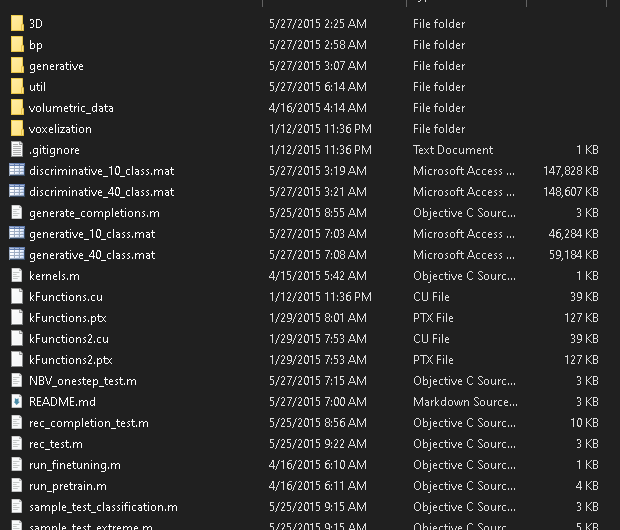
\includegraphics[scale=0.5]{figures/1174070/8/3dsnap.png}
	\caption{Isi dari dataser.zip}
\end{figure}

\end{itemize}

\subsubsection{Jelaskan apa itu voxel dengan ilustrasi dan bahasa paling awam}
\hfill\\
Secara singkat, voxel dapat diartikan sebagai 3D pixel atau pixel dalam bentuk 3D. seperti pada ilustrasi berikut:
\begin{figure}[H]
	\centering
	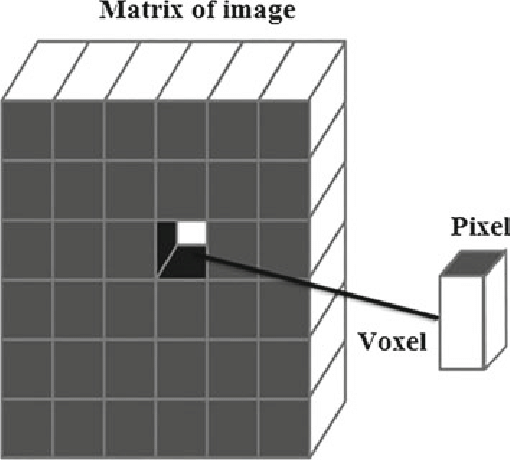
\includegraphics[width=12cm]{figures/1174070/8/voxel.png}
	\caption{Pixel VS Voxel}
\end{figure}


\subsubsection{Visualisasikan dataset tersebut dalam tampilan visual plot, jelaskan cara melakukan visualisasinya}
\hfill\\
\lstinputlisting[firstline=8, lastline=23]{src/1174070/8/praktek.py}
Kode diatas berfungsi untuk melakukan visualisasi dataset dalam tampilan plot. dengan tahapan import library, load data file .mat, dan lakukan read memakai matplotlib. dan hasilnya seperti berikut


\subsubsection{Buka file run.py jelaskan perbaris kode pada fungsi untuk membuat generator yaitu build generator}
\hfill\\
\lstinputlisting[firstline=35, lastline=41]{src/1174070/8/run.py}
potongan kode diatas berfungsi sebagai penentuan nilai untuk hyperparameters yang berbeda.
\lstinputlisting[firstline=43, lastline=43]{src/1174070/8/run.py}
potongan kode diatas berfungsi untuk membuat input layer
\lstinputlisting[firstline=45, lastline=50]{src/1174070/8/run.py}
potongan kode diatas berfungsi untuk menambahkan 3D transpose pertama.
\lstinputlisting[firstline=52, lastline=58]{src/1174070/8/run.py}
potongan kode diatas berfungsi untuk menambahkan empat 3D transpose lainya.
\lstinputlisting[firstline=60, lastline=60]{src/1174070/8/run.py}
potongan kode diatas berfungsi untuk membuat model keras dan menentukan input dan output untuk network generator.

\subsubsection{jelaskan juga fungsi untuk membangun diskriminator pada fungsi build discriminator.}
\hfill\\
\lstinputlisting[firstline=68, lastline=74]{src/1174070/8/run.py}
potongan kode diatas berfungsi sebagai penentuan nilai untuk hyperparameters yang berbeda.
\lstinputlisting[firstline=78, lastline=78]{src/1174070/8/run.py}
potongan kode diatas berfungsi untuk membuat input layer, berupa gambar 3D dengan dimensi 64x64x64x1
\lstinputlisting[firstline=80, lastline=86]{src/1174070/8/run.py}
potongan kode diatas berfungsi untuk menambahkan 3D transpose pertama.
\lstinputlisting[firstline=88, lastline=98]{src/1174070/8/run.py}
potongan kode diatas berfungsi untuk menambahkan empat 3D transpose lainya.
\lstinputlisting[firstline=100, lastline=100]{src/1174070/8/run.py}
potongan kode diatas berfungsi untuk membuat model keras dan menentukan input dan output untuk network generator.

\subsubsection{jelaskan apa maksud dari kode program name == ' main '}
\hfill\\
\lstinputlisting[firstline=153, lastline=153, caption={Kode program run.py},captionpos=b]{src/1174070/8/run.py}
maksudnya kode tersebut memiliki fungsi jika interpreter python menjalankan kode tersebut,  maka akan menetapkan variable name untuk memiliki nilai main. jika file ini di import dari modul lain, maka name akan ditetapkan ke nama modul tersbut.

\subsubsection{jelaskan secara detil perbaris dan per parameter apa arti dari kode program :}
\hfill\\
Penjelasan kode:
\lstinputlisting[firstline=157, lastline=167, caption={Kode program run.py},captionpos=b]{src/1174070/8/run.py}


\subsubsection{Jelaskan secara detil dari kode program pembuatan dan kompilasi arsitektur berikut :}
\hfill\\
\lstinputlisting[firstline=173, lastline=180, caption={Kode program run.py},captionpos=b]{src/1174070/8/run.py}
penjelasanya ialah membuat model dari generator model dan diskriminator model,


\subsubsection{Jelaskan secara detil kode program untuk membuat dan melakukan kompilasi model adversarial berikut:}
\hfill\\
\lstinputlisting[firstline=182, lastline=189, caption={Kode program run.py},captionpos=b]{src/1174070/8/run.py}
penjelasanya ialah membuat model diskriminator tidak di training dan membuat model adversarial.


\subsubsection{Jelaskan Ekstrak dan load data kursi dengan menggunakan fungsi getVoxelsFormat dan get3DImages yang digunakan pada kode program berikut :}
\hfill\\
\lstinputlisting[firstline=191, lastline=195, caption={Kode program run.py},captionpos=b]{src/1174070/8/run.py}
penjelasanya ialah melakukan print loading data, membuat variabel volumes untuk mendapatkan data gamabr 3D. 


\subsubsection{Jelaskan maksud dari kode program instansiasi TensorBoard yang menambahkan generator dan diskriminator pada program berikut:}
\hfill\\
\lstinputlisting[firstline=197, lastline=200, caption={Kode program run.py},captionpos=b]{src/1174070/8/run.py}
penjelasanya ialah membuat variabel tensorboard untuk melakukan pencatatan log, dan men-set model generator dan model diskriminator


\subsubsection{Jelaskan apa fungsi dari np reshape ones zeros pada kode program berikut dengan parameternya:}
\hfill\\
Penjelasan kode:
\lstinputlisting[firstline=202, lastline=204, caption={Kode program run.py},captionpos=b]{src/1174070/8/run.py}
membuat label\_real untuk menetapkan bahwa jika output 1 itu menunjukan gambar real, dan label\_fake untuk menunjukan bahwa output 0 untuk data fake/palsu.

\subsubsection{Jelaskan kenapa harus ada perulangan dalam meraih epoch. Dan jelaskan apa itu epoch terkait kode program berikut:}
\hfill\\
\lstinputlisting[firstline=206, lastline=212, caption={Kode program run.py},captionpos=b]{src/1174070/8/run.py}
melakukan perulangan jika MODE = train maka akan diulangi terus menerus sampai epoch(periode) terpenuhi dengan disertai keterangan generator dan diskriminator losses.

\subsubsection{Jelaskan apa itu batches dan kaitannya dengan kode program berikut, dan kenapa berada di dalam epoch:}
\hfill\\
\lstinputlisting[firstline=214, lastline=218, caption={Kode program run.py},captionpos=b]{src/1174070/8/run.py}
menghitung jumlah batch yang telah ditrain

\subsubsection{Berikut adalah kode program pengambilan gambar dan noise. Jelaskan apa fungsi np.random.normal serta astype, serta jelaskan apa arti parameter titik dua dan jelaskan isi dari z sample dan volumes batch:}
\hfill\\
\lstinputlisting[firstline=220, lastline=222, caption={Kode program run.py},captionpos=b]{src/1174070/8/run.py}
untuk membersihkan gambar dari noise dan menyesuaikan shape.

\subsubsection{Berikut adalah kode program generator gambar palsu. Jelaskan apa fungsi generator.predict on batch, serta jelaskan apa arti parameter z sample:}
\hfill\\
\lstinputlisting[firstline=224, lastline=226, caption={Kode program run.py},captionpos=b]{src/1174070/8/run.py}
untuk meng-generate volume menggunakan model jaringan generator.


\subsubsection{Berikut adalah kode program training diskriminator dengan gambar palsu dari generator dan gambar asil. Jelaskan apa maksudnya harus dilakukan training diskriminator secara demikian dan jelaskan apa isi loss fake dan loss real serta d loss dan fungsi train on batch.}
\hfill\\
\lstinputlisting[firstline=232, lastline=242, caption={Kode program run.py},captionpos=b]{src/1174070/8/run.py}
untuk membuat diskriminator bisa meload gambar fake dan real dari model generator. dengan disertai genrator dan diskriminator loss, agar terliaht seberapa baik kualitas yang dihasilkan.


\subsubsection{Berikut adalah kode program training model adversarial yang terdapat generator dan diskriminator. Jelaskan apa bagaimana proses terbentuknya parameter z dan g loss:}
\hfill\\
\lstinputlisting[firstline=244, lastline=254, caption={Kode program run.py},captionpos=b]{src/1174070/8/run.py}
untuk mentrain model generator dan variabel g\_loss untuk melakukan perbandingan antara label gambar yang asli.

\subsubsection{Berikut adalah kode program generate dan menyimpan gambar 3D setelah beberapa saat setiap epoch. Jelaskan mengapa ada perulangan dengan parameter tersebut, serta jelaskan arti setiap variabel beserta perlihatkan isinya dan artikan isinya :}
\hfill\\
\lstinputlisting[firstline=256, lastline=265, caption={Kode program run.py},captionpos=b]{src/1174070/8/run.py}
untuk melakukan perulangan dimana setiap terdapat 10 mini-batch akan meng-generate volumenya dan akan menyimpannya.


\subsubsection{Berikut adalah kode program menyimpan average losses setiap epoch. Jelaskan apa itu tensorboard dan setiap parameter yang digunakan pada kode program ini :}
\hfill\\
\lstinputlisting[firstline=267, lastline=270, caption={Kode program run.py},captionpos=b]{src/1174070/8/run.py}
untuk menuliskan log losses ke Tensorboard

\subsubsection{Berikut adalah kode program menyimpan model. Jelaskan apa itu format h5 dan penjelasan dari kode program berikut :}
\hfill\\
\lstinputlisting[firstline=276, lastline=278, caption={Kode program run.py},captionpos=b]{src/1174070/8/run.py}
untuk menyimpan berat model generator dan model diskriminator kedalam file h5.

H5 adalah Hierarchical Data Format 5 File.
File H5 adalah file data yang disimpan dalam Format Data Hirarki (HDF). Ini berisi array multidimensi data ilmiah. File H5 biasanya digunakan di luar angkasa, fisika, teknik, keuangan, penelitian akademis, genomik, astronomi, instrumen elektronik, dan bidang medis.

\subsubsection{Berikut adalah kode program testing model. Jelaskan dengan ilustrasi gambar dari mulai meload hingga membuat gambar 3D dengan menggunakan z sample, bisakah parameter z sample tersebut diubah2? :}
\hfill\\
\lstinputlisting[firstline=287, lastline=298, caption={Kode program run.py},captionpos=b]{src/1174070/8/run.py}
untuk membuat mode predict/prediksi. dimana dia melakukan pebuatan model generator, model diskriminator dan meload data h5 yang sudah dibuat tadi dan meng-generate nya kedalam model 3D, lalu menyimpan model voxel nya ke folde results.

\subsection{Penanganan Error}
\subsubsection{Terjadi error}
\hfill\\
\begin{enumerate}
\item terjadi error Summary has no attribute, seperti pada gambar berikut:
\end{enumerate}

\subsubsection{Solusi}
\hfill\\
\begin{enumerate}
\item solusi dari error 1 ialah:
dengan menginstall versi tensorflow 1.xx

\end{enumerate}

\subsection{Bukti Tidak Plagiat}
\begin{figure}[H]
	\centering
	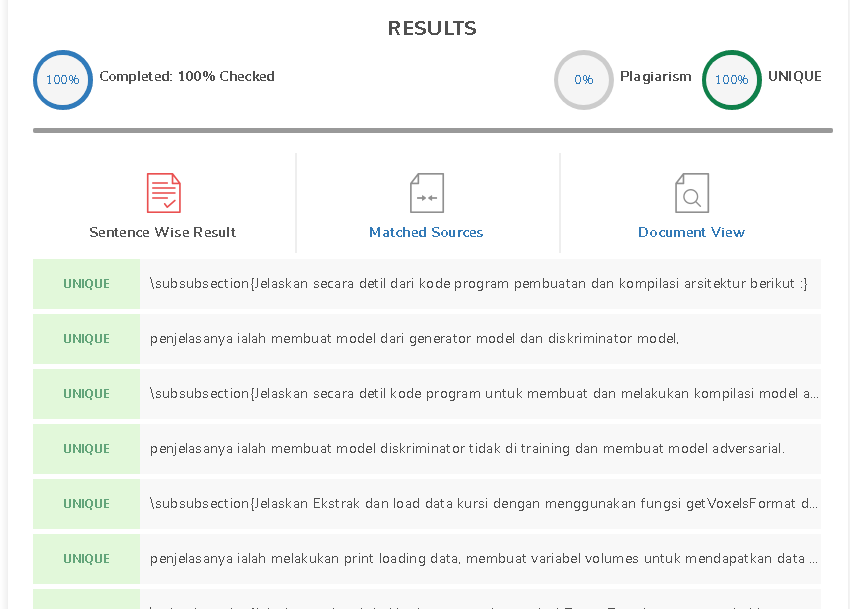
\includegraphics[width=12cm]{figures/1174070/8/plagiat.png}
	\caption{Bukti tidak plagiat}
\end{figure}

